\documentclass[12pt]{article}
\usepackage[utf8]{inputenc}
\usepackage{graphicx}
\usepackage{amsmath}
\usepackage{hyperref}
\usepackage{subcaption}

\title{Modeling and Simulation of Earth's Average Global Temperature}
\author{Palmisano Luca \\ Bourgeois Noé}
\date{November 2023}

\begin{document}

\maketitle

\begin{abstract}
\noindent
The present report outlines the findings from a series of simulations designed to model the Earth's average global temperature. Utilizing a range of models, from a basic Energy Balance Model (EBM) to more complex variations incorporating factors like albedo and emissivity, this study aims to provide insights into the dynamics of Earth's climate system and the factors influencing its temperature.
\end{abstract}

\section{Introduction}
Climate change, characterized by alterations in Earth's average temperature, is a critical global issue. This report focuses on modeling the Earth's temperature using various simulation models. The objective is to understand how different parameters affect global temperature. We explore several models, including the Basic EBM and its extensions, to simulate and analyze temperature changes under different conditions.

\section{Methodology}
The methodology employed in this project involves simulating Earth's temperature using several models. The Basic EBM is the starting point, which is then expanded to include factors like albedo variation and emissivity. The simulations are conducted using the Octave software, leveraging its numerical computation capabilities to solve complex differential equations inherent in the models.

\section{Results}
% Fill in your simulation results here.
% Use graphs and tables to present your data.
% Example of including a figure:

\subsection{Basic EBM}
The equilibrium temperature of the system in the basic Energy Balance Model (EBM) is calculated by balancing the incoming solar radiation with the outgoing longwave radiation. This balance is represented by the equation:

\begin{equation}
Q(1 - \alpha) = \sigma T_{eq}^4
\end{equation}

where:
\begin{itemize}
    \item $Q$ is the average global solar radiation (342 W/m$^2$).
    \item $\alpha$ is the albedo of the planet (0.3).
    \item $\sigma$ is the Stefan-Boltzmann constant ($5.67 \times 10^{-8}$ W/m$^2$/K$^4$).
    \item $T_{eq}$ is the equilibrium temperature in Kelvin.
\end{itemize}

Rearranging the equation to solve for $T_{eq}$, we get:

\begin{equation}
T_{eq} = \left( \frac{Q(1 - \alpha)}{\sigma} \right)^{\frac{1}{4}}
\end{equation}

Substituting the values:

\begin{equation}
T_{eq} = \left( \frac{342 \times (1 - 0.3)}{5.67 \times 10^{-8}} \right)^{\frac{1}{4}}
\end{equation}

Calculating this, we find:

\begin{equation}
T_{eq} \approx 254.91 \, \text{K}
\end{equation}

This is the theoretical equilibrium temperature of the Earth according to this simple model, which does not account for the greenhouse effect.


\begin{figure}[ht]
\centering
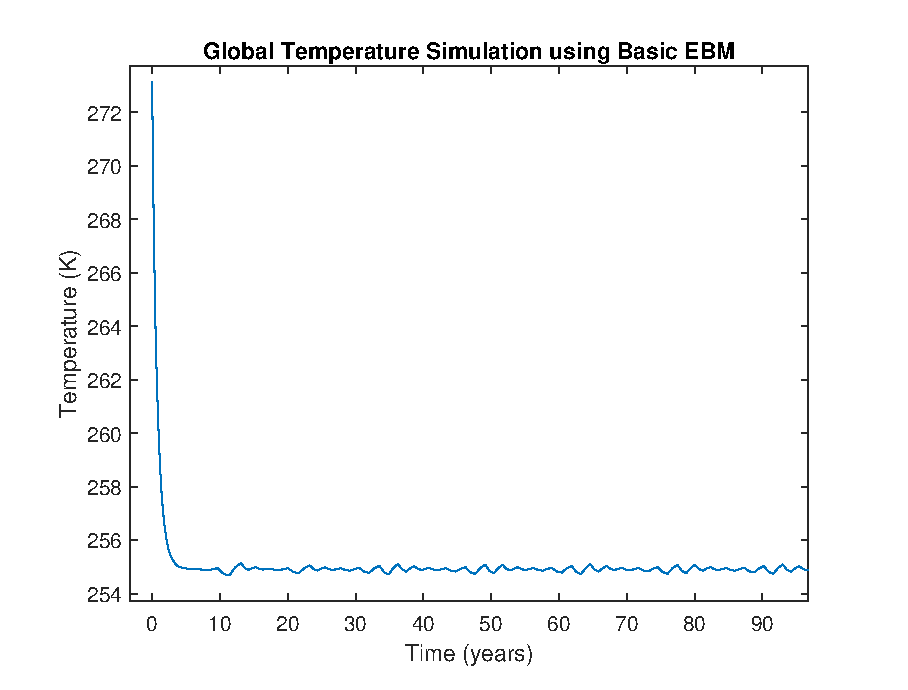
\includegraphics[width=0.8\textwidth]{ebm_basic.eps}
\caption{Simulation results for the Basic EBM model.}
\label{fig:basicEBM}
\end{figure}

\subsubsection{Albedo Variation}
The albedo of the Earth is not constant, 
and varies with the seasons. 
The albedo is higher in the winter due to the presence of snow and ice, 
and lower in the summer due to the presence of vegetation. 

For an albedo ($\alpha$) of 0 (absorbing all incoming solar radiation), 
the equilibrium temperature is approximately 278.68 Kelvin.
For an albedo of 1 (reflecting all incoming solar radiation), 
the equilibrium temperature is 0 Kelvin.
These results highlight the significant impact of albedo on the Earth's temperature. 
An albedo of 1 is an extreme and theoretical scenario 
where all incoming solar radiation is reflected, 
leading to no energy absorption 
and hence a theoretical equilibrium temperature of absolute zero. 
In contrast, an albedo of 0 leads to higher temperatures 
due to the absorption of all incoming solar radiation. 

\begin{figure}[ht]
\centering
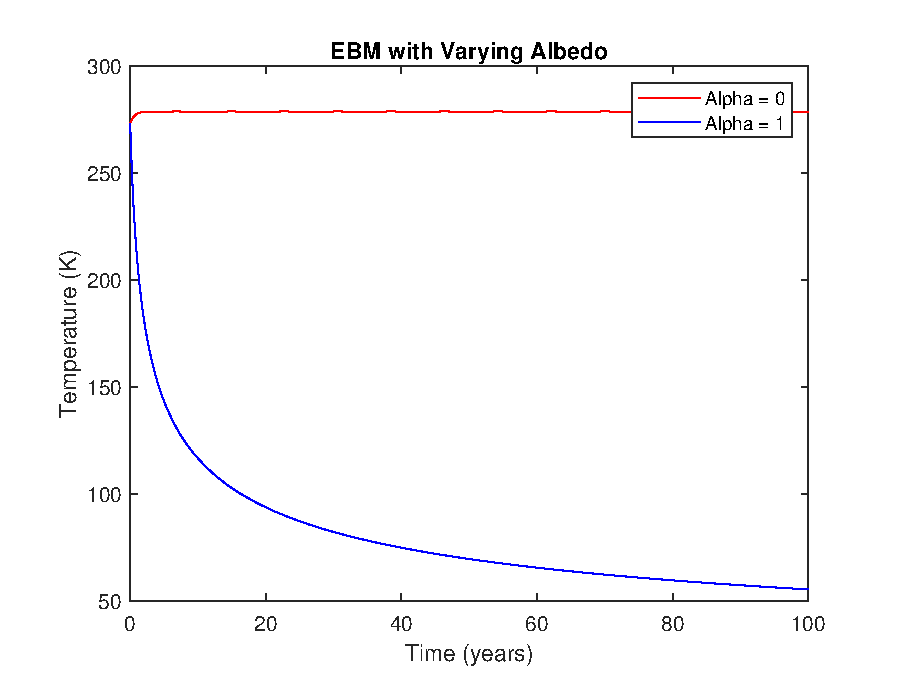
\includegraphics[width=0.8\textwidth]{albedo_extremes.eps}
\caption{Simulation results for the Basic EBM model with albedo extremes.}
\label{fig:albedoExtremes}
\end{figure}

\subsubsection{Emissivity}
The equilibrium temperature of the system, 
considering emissivity in the Energy Balance Model (EBM), 
is calculated by modifying the original equation 
to include the emissivity factor. 

The modified equation at equilibrium is:

\begin{equation}
0 = Q(1 - \alpha) - \epsilon\sigma T_{eq}^4
\end{equation}

Rearranging this equation to solve for the equilibrium temperature ($T_{eq}$):

\begin{equation}
\epsilon\sigma T_{eq}^4 = Q(1 - \alpha)
\end{equation}

\begin{equation}
T_{eq}^4 = \frac{Q(1 - \alpha)}{\epsilon\sigma}
\end{equation}

\begin{equation}
T_{eq} = \left( \frac{Q(1 - \alpha)}{\epsilon\sigma} \right)^{\frac{1}{4}}
\end{equation}

Substituting the values:
\begin{itemize}
    \item $Q = 342 \, \text{W/m}^2$ (Average global solar radiation).
    \item $\alpha = 0.3$ (Albedo).
    \item $\sigma = 5.67 \times 10^{-8} \, \text{W/m}^2/\text{K}^4$ (Stefan-Boltzmann constant).
    \item $\epsilon = 0.61$ (Emissivity, a typical value for Earth).
\end{itemize}

The equilibrium temperature ($T_{eq}$) is calculated as:

\begin{equation}
T_{eq} = \left( \frac{342 \times (1 - 0.3)}{0.61 \times 5.67 \times 10^{-8}} \right)^{\frac{1}{4}} \approx 288.44 \, \text{K}
\end{equation}

This equilibrium temperature is much closer to the actual average surface temperature of the Earth, demonstrating the significant impact of emissivity in the energy balance model.


\begin{figure}[ht]
    \centering
    \begin{subfigure}[b]{0.4\textwidth}
        \centering
        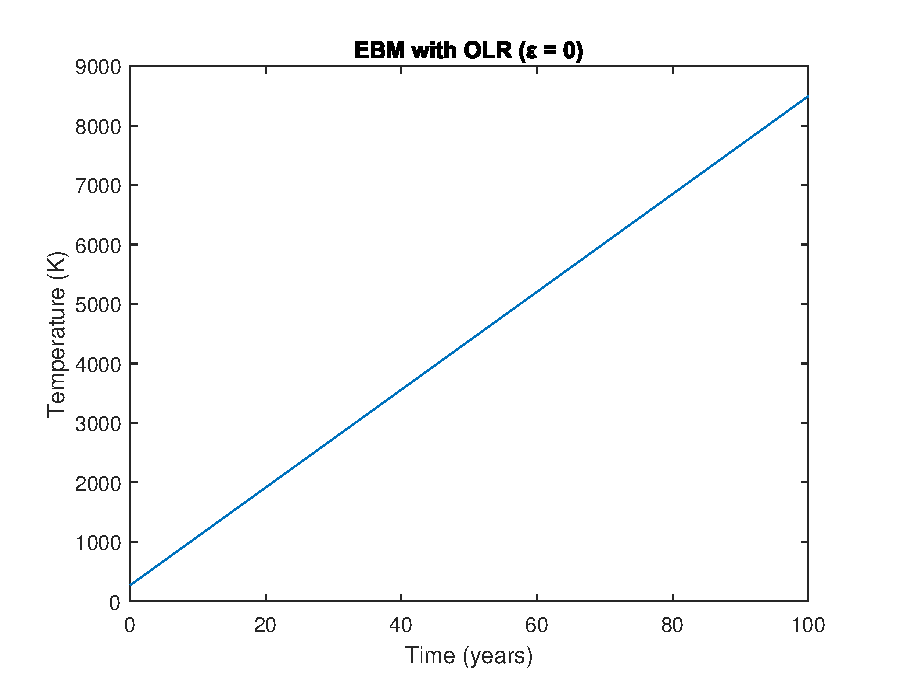
\includegraphics[width=\textwidth]{ebm_with_olr_0.eps}
            \caption{First subfigure}
        \label{fig:sub1}
    \end{subfigure}
    \hfill % Adds horizontal space between the subfigures
    \begin{subfigure}[b]{0.4\textwidth}
        \centering
        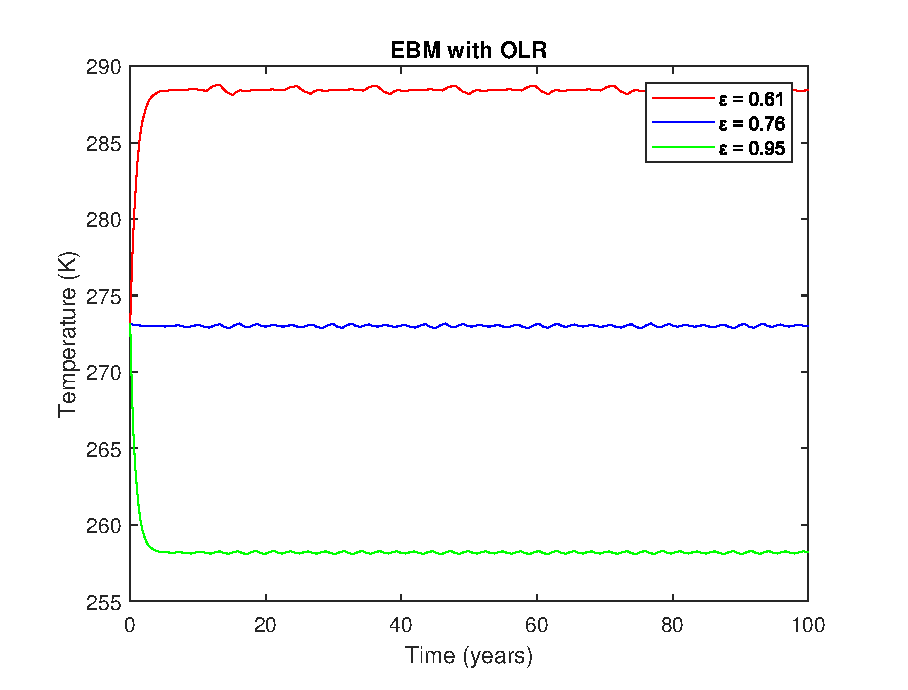
\includegraphics[width=\textwidth]{ebm_with_diff_olrs.eps}
        \caption{Second subfigure}
        \label{fig:sub2}
    \end{subfigure}
    \caption{Overall figure caption}
    \label{fig:test}
\end{figure}

\section{Discussion}
% Analyze the results you've presented.
% How do the models compare with each other?
% Discuss the implications of your findings, especially in the context of climate change.
% Are there any limitations or notable aspects of the models that affected the results?

\section{Conclusion}
% Summarize your main findings.
% Reflect on what these results mean for our understanding of Earth's climate system.

\end{document}
